\begin{tikzpicture}[scale=0.35,thick] % , baseline = -3.5pt


\only<1>{\draw (0,-3)--(0,-5) node[midway,right] {\tiny $\catvariableof{0}$}; }
\only<2->{\draw (0,-3)--(0,-4) node[midway,right] {\tiny $\catvariableof{0}$}; }

\only<1->{

\draw (-1,-1) rectangle (5,-3);
\node[anchor=center] (text) at (2,-2) {\small $\hypercoreof{\edge_1}$};


\draw (2,-3)--(2,-5) node[midway,right] {\tiny $\catvariableof{1}$};
\draw (4,-3)--(4,-5) node[midway,right] {\tiny $\catvariableof{2}$};


\draw (6,-1) rectangle (10,-3);
\node[anchor=center] (text) at (8,-2) {\small $\hypercoreof{\edge_3}$};
\draw (7,-3)--(7,-5) node[midway,right] {\tiny $\catvariableof{2}$};
\draw (9,-3)--(9,-5) node[midway,right] {\tiny $\catvariableof{3}$};

\begin{scope}[shift={(0,-2)}]
\draw (1,-7) rectangle (5,-9);
\node[anchor=center] (text) at (3,-8) {\small $\hypercoreof{\edge_2}$};
\draw (2,-5)--(2,-7) node[midway,right] {\tiny $\catvariableof{1}$};
\draw (4,-5)--(4,-7) node[midway,right] {\tiny $\catvariableof{2}$};

\end{scope}
}

\only<2->{
\draw (2,-5)--(2,-7);

\draw (4,-5) to[bend right=20]  (7,-6); % node[midway,left] {\tiny $\catvariableof{2}$};
\draw (4,-7) to[bend right=-20]  (7,-6); 

\draw[fill] (2,-6) circle (0.25cm);
\draw (2,-6) to[bend right=20] (-1,-8); % node[midway, right]{\tiny $\catvariableof{1}$};
\node[anchor=center] (text) at (-2,-8) {\tiny $\catvariableof{1}$};

\draw[fill] (7,-6) circle (0.25cm);
\draw (7,-5) -- (7,-6);
\draw (7,-6)--(7,-7) node[midway,right] {\tiny $\catvariableof{2}$};


\draw (-1,-4) rectangle (1,-6);
\node[anchor=center] (text) at (0,-5) {\small $\ones$};
\draw (6,-7) rectangle (8,-9);
\node[anchor=center] (text) at (7,-8) {\small $\ones$};
}



\end{tikzpicture}